\setcounter{equation}{0}
\addcontentsline{toc}{chapter}{\numberline{}Curriculum Vitae}

\thispagestyle{plain}
\renewcommand{\chaptermark}[1]{ \markboth{#1}{} }
\renewcommand{\sectionmark}[1]{ \markright{#1} }
\renewcommand{\headrulewidth}{0.4pt} % remove lines as well
\renewcommand{\footrulewidth}{0.4pt}
\fancyhead[LE]{\textit{\nouppercase{Curriculum Vitae}} }
\fancyhead[RO]{\textit{\nouppercase{Curriculum Vitae}} }
\fancyfoot[RO,LE]{\thepage}

\chapter*{Curriculum Vitae}
\center 
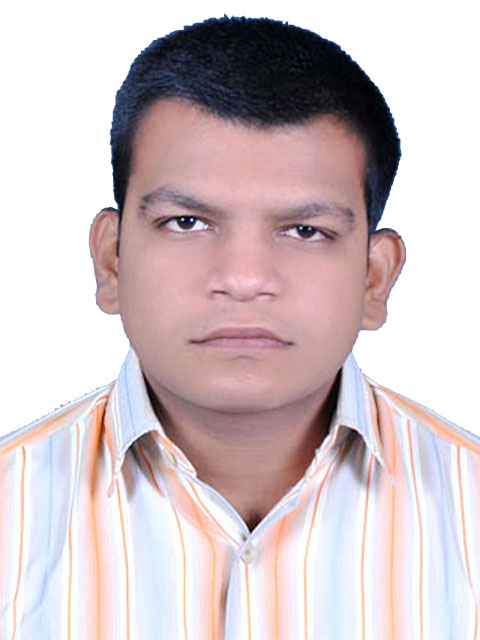
\includegraphics[scale=0.2]{figures/sohanpande.jpg}
\justify
\textbf{Mr. Sohan Kumar Pande} was born to Mr. Kanhu Charan Pande and Mrs. Pravati Pradhan on 10 June 1990 in Sambalpur, Odisha, India. He completed his matriculation with 83.33\% from Budharaja High School, Sambalpur in the year 2005 and +2 Science with 68.33\% from G. M. Junior College, Sambalpur in the year 2007. He obtained his B. Tech. Degree in Computer Science and Engineering with 7.29 CGPA from C. V. Raman College of Engineering, Bhubaneswar, Odisha, India, in the year 2012 and M. Tech. Degree in Computer Science with 9.3 CGPA from Sambalpur University Institute of Information Technology, Odisha, India, in the year 2016. He is currently pursuing his Ph.D. in the Department of Computer Science and Engineering at Veer Surendra Sai University of Technology, Burla, Odisha, India, under the guidance of Dr. Satyabrata Das, Associate Professor, Department of IT, VSSUT, Burla and Dr. Sanjaya Kumar Panda, Assistant Professor, Department of CSE, NIT, Warangal. He has got experience in multiple reputed institutions with various roles, such as guest faculty in the Department of MCA G. M. Autonomous College, Sambalpur, Odisha, India, from the year 2012 to 2015. Then, he worked in the Department of BCA, Vikash School Of Business Management, Bargarh, Odisha, India, as an Assistant Professor from 2017 to 2019. Currently, he is working as an Assistant Professor in the Department of Computer Science and Engineering, Silicon Institute of Technology, Sambalpur, Odisha, India, since 2019.  He is also an Academic Counselor at Odisha State Open University, Sambalpur, Odisha, since 2016 and Program-in-Charge since 2019. Besides, he has developed websites for various organizations. He has published more than ten papers in reputed journals and conferences. He acted as a reviewer in many reputed journals and conferences. He has also got the Sandeep Mohapatra Memorial Award, The Institute of Engineers (India), Odisha State Center, Bhubaneswar. His current research interests include vehicular clouds, cloud computing, grid computing and load balancing. \\
\begin{flushleft}
\textbf{Communication Details} \\
\begin{tabular}{rl}
	Permanent Address: & Mr. Sohan Kumar Pande                                                                                                                          \\
	& \begin{tabular}[c]{@{}l@{}}S/O - Kanhu Charan Pande\\ Matru Vihar (Danipali),\\ Budharaja-768004, \\ Sambalpur, Odisha, INDIA\end{tabular} \\
	Email:             & ersohanpande@gmail.com                                                                                           \\
	Mobile No.:        & +91-9777339851                                                                                                                                
\end{tabular}
\end{flushleft}